% Integration fragment; uses amsmath, amssymb, amsthm.
% Source: Balitskiy--Mitrofanov--Polyanskii, arXiv:2603.12495v2
% (19 August 2026), Theorem 3.3, Section 6.2, Conjecture 6.1.
\section{Truncated parallelograms: strict Viterbo and competing covers}
\label{sec:truncated-square-cover}

Balitskiy, Mitrofanov and Polyanskii conjectured a particular optimal
trapezoidal partner for every square with one corner truncated
\cite[Section~6.2, Conjecture~6.1]{BMP2026}. We construct a different
trapezoidal partner which improves their proposed optimum on an open set
of truncation parameters. This disproves the optimizer assertion of that
conjecture. We first prove its strict-inequality assertion for every convex
partner, so the two assertions have different outcomes.

We use their normal-triangle covering theorem
\cite[Theorem~3.3]{BMP2026}: for a polygon $Q$, the inequality
$c_{\mathrm{EHZ}}(K\times_L Q)\geq1$ is equivalent to $K$ containing a
translate of each $Q$-normal triangle of unit $Q$-perimeter. Degenerate
triangles, namely segments traversed in both directions, are included.
The $Q$-perimeter of a closed polygonal curve with directed edge vectors
$e_i$ is $\sum_i h_Q(e_i)$, where $h_Q$ denotes the support function.
This quantity is unchanged by translating $Q$.

Choose
\[
 0<A,B<1,\qquad g=A+B-1>0,\qquad a=1-A,\qquad d=B-a^2.
\]
In particular $B>a$ and $d>0$. Put $r=g/B$ and $s=g/A$, and define
\[
 Q_{A,B}=\operatorname{conv}\{(0,0),(1,0),(1,1-r),(1-s,1),(0,1)\}.
\]
Both $r,s$ belong to $(0,1)$, so this is a genuine corner-truncated
square. Its area is
\begin{equation}\label{eq:truncated-Q-area}
 |Q_{A,B}|=1-\frac{rs}{2}=1-\frac{g^2}{2AB}.
\end{equation}

The outward-normal directions of $Q_{A,B}$ are
$\pm e_1,\pm e_2,(r,s)$. The only nondegenerate positively dependent
triple is $-e_1,-e_2,(r,s)$; the only minimal positive pairs are the two
opposite coordinate pairs. Consequently its complete list of unit normal
templates, up to translation, consists of
\begin{equation}\label{eq:four-truncated-templates}
 T=\operatorname{conv}\{(0,0),(A,0),(A,B)\},\quad -T,\quad
 H=[0,e_1],\quad V=[0,e_2].
\end{equation}
For completeness, traverse $T$ in the order $(A,B),(A,0),(0,0)$.
Its edge directions are
\[ -e_2,\quad -e_1,\quad(r,s), \]
 and its $Q_{A,B}$-perimeter
is one: the first two support-function contributions vanish, while
$h_{Q_{A,B}}(A,B)=1$, because the cut line is
$rx+sy=r+s-rs=g/(AB)$ and $(A,B)=(AB/g)(r,s)$.
The two coordinate segments have unit perimeter because $Q_{A,B}$ has
unit width in both coordinate directions. Reversing the order of the three
edge directions gives the translation class $-T$.

% Insert after defining Q_{A,B} and its four templates, before the new cover.
% Uses the notation A,B,g and labels in truncated-square-section.tex.
\subsection{The Viterbo inequality for all partners}

The covering description also proves the Viterbo inequality for the entire
corner-truncated-square class, independently of which cover has minimum area.

\begin{theorem}\label{thm:truncated-global-viterbo}
Let $Q\subset\mathbb R^2$ be a parallelogram with one corner cut off by a
line meeting the interiors of its two adjacent sides. For every planar
convex body $K$ with nonempty interior,
\[
 c_{\mathrm{EHZ}}(K\times_L Q)^2<2|K|\,|Q|.
\]
In the normalization $Q=Q_{A,B}$ above, every capacity-one cover satisfies
\begin{equation}\label{eq:truncated-global-area}
 |K|>\frac{AB}{2AB-(A+B-1)^2}.
\end{equation}
Thus the strict-inequality assertion of \cite[Conjecture~6.1]{BMP2026}
holds, although its proposed optimizer will be disproved below.
\end{theorem}

\begin{proof}
An affine change in the $Q$-plane, paired with its inverse transpose in
the $K$-plane, reduces to $Q_{A,B}$ without changing the capacity or the
product of areas. Scaling $K$, we may assume its product capacity is one.
It therefore contains translated copies of the four templates
$T,-T,H,V$ from \eqref{eq:four-truncated-templates}.

First, this implies a lattice covering property. Put
\[
 \Lambda=A\mathbb Z e_1+B\mathbb Z e_2.
\]
Split every fundamental rectangle by its diagonal parallel to $(A,B)$.
The resulting triangulation has cells that are translates of $T$ or $-T$.
We use the triangulation-covering lemma
\cite[Lemma~4.3]{BMP2026}: if every cell of a planar triangulation fits by
translation into a convex body, then every translate of that body meets
the vertex set of the triangulation. It follows that
\begin{equation}\label{eq:truncated-lattice-cover}
 K+\Lambda=\mathbb R^2.
\end{equation}

Suppose first that $K$ contains a translate of the axis-parallel rectangle
$[0,A]\times[0,B]$. Let $w_x,w_y$ be the coordinate widths of $K$.
The four caps based on the rectangle's sides and reaching support-maximizing
points of $K$ have pairwise disjoint interiors
\cite[Lemma~7.1]{BMP2026}. Adding their areas to the rectangle's area gives
\[
 |K|\geq AB+\frac B2(w_x-A)+\frac A2(w_y-B)
       =\frac{Bw_x+Aw_y}{2}\geq\frac{A+B}{2},
\]
because $H,V$ fit into $K$ and hence $w_x,w_y\geq1$.
The cap lemma applies to an arbitrary convex body: only the four support
maximizers and the rectangle are used, so one may equivalently apply its
polygonal statement to their convex hull. This branch is strictly stronger
than the desired bound, since
\[
 \frac{A+B}{2}-\frac{AB}{2AB-g^2}
 =\frac{g\bigl(A(1-A)+B(1-B)\bigr)}{2(2AB-g^2)}>0.
\]

Now suppose no translate of that rectangle is contained in $K$.
For each $t\in\mathbb R^2$, form a finite graph whose vertices are
$(K-t)\cap\Lambda$, joining two vertices when their difference is
$Ae_1$ or $Be_2$. It is nonempty by \eqref{eq:truncated-lattice-cover}.
It is also a forest. Indeed, a cycle contains a simple rectilinear cycle;
its bounded interior contains a fundamental lattice cell. The closure of
that cell lies in the convex hull of the cycle vertices, hence in $K-t$.
This would put a translate of $[0,A]\times[0,B]$ inside $K$, contrary
to the present assumption. Thus, writing $N(t)$ for the number of vertices
and $E_x(t),E_y(t)$ for the two types of edges,
\[
 E_x(t)+E_y(t)\leq N(t)-1.
\]
Integrate this inequality over a fundamental rectangle of $\Lambda$.
Periodization of indicator functions gives
\[
 \int N(t)\,dt=|K|,\qquad
 \int E_x(t)\,dt=|K\cap(K+Ae_1)|,\qquad
 \int E_y(t)\,dt=|K\cap(K+Be_2)|.
\]
The fundamental rectangle has area $AB$, so
\begin{equation}\label{eq:forest-overlap}
 |K|-AB\geq |K\cap(K+Ae_1)|+|K\cap(K+Be_2)|.
\end{equation}

Finally, let $[u,u+e_1]\subset K$ be a placed copy of $H$.
Convexity gives the homothetic inclusion
\[
 (1-A)K+A(u+e_1)\subset K\cap(K+Ae_1),
\]
because subtracting $Ae_1$ from the left-hand side gives
$(1-A)K+Au\subset K$. Consequently
\[
 |K\cap(K+Ae_1)|\geq(1-A)^2|K|.
\]
The placed copy of $V$ gives the analogous bound
$|K\cap(K+Be_2)|\geq(1-B)^2|K|$. Inserting these inequalities
into \eqref{eq:forest-overlap} yields
\[
 \bigl(1-(1-A)^2-(1-B)^2\bigr)|K|\geq AB.
\]
The coefficient on the left equals $2AB-g^2>0$, which proves
the weak form of \eqref{eq:truncated-global-area}. Together with
$|Q_{A,B}|=(2AB-g^2)/(2AB)$, this proves the weak capacity-volume
inequality for every partner.

It remains to exclude equality. Suppose $|K|=AB/(2AB-g^2)$.
Replace $K$ by the convex hull $P$ of one placed copy of each of the four
templates. This polygon has at most ten vertices, is contained in $K$,
and still has product capacity at least one. The weak inequality already
proved gives $|P|\geq AB/(2AB-g^2)=|K|$, hence $P=K$.
Thus an equality body is a polygon. The rectangle case was strict, so
equality must hold in the two homothetic overlap inclusions. In particular,
with $[u,v]=[u,u+e_1]\subset K$,
\begin{equation}\label{eq:overlap-set-equality}
 K\cap(K+Ae_1)=(1-A)K+Av.
\end{equation}
The equality of sets follows from their inclusion and equal areas.

Let $n$ be an outward normal of any genuine facet of $K$.
The right side of \eqref{eq:overlap-set-equality} has a genuine facet
with that normal. An edge of an intersection of polygons comes from an
edge of one of the intersected polygons. Its supporting value is therefore
$h_K(n)+A\min\{0,n\cdot e_1\}$. Comparing supporting values in
\eqref{eq:overlap-set-equality} gives
\[
 (1-A)h_K(n)+A\,n\cdot v
 =h_K(n)+A\min\{0,n\cdot e_1\},
\]
so
\[
 h_K(n)=\max\{n\cdot u,n\cdot v\}.
\]
Every facet of $K$ consequently contains at least one endpoint of the unit
horizontal segment. Each endpoint can belong to at most two genuine
facets of a planar polygon. Hence $K$ has at most four facets.

If $K$ has four facets, their coverage by the two endpoints forces $u,v$
to be opposite vertices. Applying the same argument to the vertical
overlap equality shows that the endpoints of the unit vertical segment
are the other two opposite vertices. The two diagonals are perpendicular
and both have length one, so $|K|=1/2$. This is impossible because
$AB/(2AB-g^2)>1/2$.

The only remaining case is a triangular $K$. After translation, write
\[
 K=M\operatorname{conv}\{0,e_1,e_2\},\qquad \det M\ne0.
\]
The product symmetry $c(K\times_L Q)=c(Q\times_L K)$, followed by the
inverse-transpose linear change in the other factor, shows that $M^TQ$
is a capacity-one partner of the standard triangle. Its two normal
triangles triangulate the unit square grid. Applying the same
triangulation-covering lemma therefore gives
\[
 Q+M^{-T}\mathbb Z^2=\mathbb R^2.
\]
This lattice has covolume
\[
 |\det M|^{-1}=\frac{1}{2|K|}=|Q|.
\]
A lattice cover at this exact area has multiplicity one almost everywhere:
its multiplicity is at least one and its integral over a fundamental cell
is the cell's area. In particular distinct translates have disjoint
interiors, so these translates tile the plane.

Every edge of a convex polygon that tiles by lattice translations has
another edge parallel to it with the opposite outward normal. To see this,
choose a relative-interior point of the edge which is not a vertex of any
of the locally finitely many neighboring tiles. A tile covering points
just beyond that edge must meet it in an edge with the opposite normal;
interior overlap is impossible. But the truncation edge of $Q_{A,B}$ has
no edge with the opposite normal. Thus $Q_{A,B}$ cannot be such a tile.
This contradiction excludes equality and proves the strict inequality.
\end{proof}

The argument separates two possibilities: a full lattice cell already
contained in $K$ gives a direct cap-area estimate, while its absence makes
the lattice-point graphs acyclic and converts lattice covering into an
upper bound on overlap. The unit normal segments supply the opposite,
homothetic lower bounds on those overlaps. Equality would force a partner
with at most four sides; the four-sided case has too little area, and the
triangular case would force the truncated square to tile by translations.

\subsection{A uniform gap and nearby norms}

The pointwise strict inequality has a useful uniform consequence.  Here
neighborhoods are taken in the Hausdorff topology on planar convex bodies;
translations of either factor do not affect the capacity or the area.

\begin{corollary}\label{cor:truncated-neighborhood}
Let $Q$ be a genuine corner-truncated parallelogram.  There are a constant
$\delta_Q>0$ and a neighborhood $\mathcal U_Q$ of $Q$ such that, for every
planar convex body $K$,
\[
 c_{\mathrm{EHZ}}(K\times_L Q)^2
 \le (1-\delta_Q)\,2|K|\,|Q|,
\]
and, for every $Q'\in\mathcal U_Q$,
\[
 c_{\mathrm{EHZ}}(K\times_L Q')^2<2|K|\,|Q'|.
\]
In particular, this gives open sets of admissible factors containing
pentagons without parallel sides and smooth strictly convex bodies.
\end{corollary}

\begin{proof}
Use the affine normalization and four normal templates of the preceding
proof.  Let $m_Q$ be the infimum of $|K|$ over convex bodies containing
translates of all four templates.  This infimum is finite, and the normal
cover criterion identifies the constraint with
$c_{\mathrm{EHZ}}(K\times_L Q)\ge1$.

We first check attainment.  If $K$ contains a vertical unit segment, the
triangles joining that segment to points of minimum and maximum first
coordinate have disjoint interiors.  Consequently
$\operatorname{width}_{e_1}K\le2|K|$.  The horizontal unit segment similarly
gives $\operatorname{width}_{e_2}K\le2|K|$.  A minimizing sequence with bounded
area is therefore uniformly bounded after translation.  Blaschke selection
provides a Hausdorff limit.  The four template containments persist in the
limit, since their translation vectors are bounded and may be passed to
subsequences.  In particular, the limit contains the nondegenerate triangle
$T$ and is a convex body.  Continuity of area proves that it attains $m_Q$.
The strict theorem, applied to this minimizer, gives
\[
 m_Q>\frac1{2|Q|}.
\]
Indeed its capacity is at least one.  Rescaling the first factor to capacity
one now gives the first assertion with
$\delta_Q=1-(2m_Q|Q|)^{-1}>0$.

Translate $Q$ so that the origin lies in its interior and choose
$\varepsilon\in(0,1)$ small enough that
\[
 (1-\delta_Q)\left(\frac{1+\varepsilon}{1-\varepsilon}\right)^2<1.
\]
For all $Q'$ in a sufficiently small Hausdorff neighborhood of $Q$,
\[
 (1-\varepsilon)Q\subset Q'\subset(1+\varepsilon)Q.
\]
Monotonicity and homogeneity of capacity, together with area monotonicity,
yield
\[
 \frac{c_{\mathrm{EHZ}}(K\times_L Q')^2}{2|K|\,|Q'|}
 \le
 \left(\frac{1+\varepsilon}{1-\varepsilon}\right)^2
 \frac{c_{\mathrm{EHZ}}(K\times_L Q)^2}{2|K|\,|Q|}
 <1.
\]
Small generic perturbations of the five vertices remove the parallel edge
pairs, while smooth strictly convex bodies approximate $Q$ in Hausdorff
distance.  Both therefore occur in this neighborhood.
\end{proof}

\begin{remark}
This argument establishes existence of the gap and of the neighborhood.
It gives no explicit value of $\delta_Q$ or radius of $\mathcal U_Q$, and it
does not identify the minimizing partner.
\end{remark}


\begin{theorem}\label{thm:alternative-truncated-cover}
With the preceding notation, let
\[
 D=\left(\frac{A^2a}{d},-\frac{A^2B}{d}\right),\qquad
 L=-\frac aA D,\qquad R=L+(1,0),\qquad C=(A,B),
\]
and let $K_{A,B}=\operatorname{conv}\{L,D,R,C\}$. Then
\begin{align}
 c_{\mathrm{EHZ}}(K_{A,B}\times_L Q_{A,B})&=1,
 \label{eq:alternative-capacity}\\
 |K_{A,B}|&=F(A,B):=\frac{B(2A+B-1)}{2[B-(1-A)^2]},
 \label{eq:alternative-area}\\
 \rho(K_{A,B}\times_L Q_{A,B})
 &=\frac{2Ad}{(A+g)(2AB-g^2)}<1.
 \label{eq:alternative-sys}
\end{align}
The sides $LD$ and $RC$ are parallel. Thus $K_{A,B}$ is a trapezoid.
\end{theorem}

\begin{proof}
Consider the affine-linear functions
\[
 \phi(x,y)=Bx+ay,\qquad
 U(x,y)=y-\frac gA x-a,\qquad
 G(x,y)=y-\frac{AB}{g}(x-A).
\]
Direct substitution, using $AB+ag=d$ and $d-Aa=g$, shows that
\begin{equation}\label{eq:alternative-halfplanes}
 K_{A,B}=\{(x,y):0\leq\phi(x,y)\leq B,\ U(x,y)\leq0,\ G(x,y)\geq0\}.
\end{equation}
Its successive vertices are $L,D,R,C$: $LD$ and $RC$ lie on the
parallel lines $\phi=0$ and $\phi=B$, respectively; $LC$ lies on
$U=0$ and $DR$ on $G=0$. All four sides have positive length under
the stated strict inequalities.

We exhibit placements of the four templates in
\eqref{eq:four-truncated-templates}. The triangle $T$ is already contained
in $K_{A,B}$. Indeed the values of $(\phi,U,G)$ at its successive vertices
$(0,0),(A,0),(A,B)$ are
\[
 (0,-a,A^2B/g),\qquad (AB,-B,0),\qquad (B,0,B),
\]
which satisfy \eqref{eq:alternative-halfplanes}. The horizontal segment
is $L+H=[L,R]$. The vertical segment is $D+V$: at $D$ its three values
are $(0,-1,0)$, and at $D+e_2$ they are $(a,0,1)$. Here $0<a<B$.

For the opposite triangle, put
\[
 t=\left(A+\frac{aAg}{d},\frac{aB(A+g)}d\right).
\]
The values of $(\phi,U,G)$ at the vertices
$t,t-(A,0),t-(A,B)$ of $-T+t$ are, respectively,
\[
 \begin{array}{c|ccc}
 &\phi&U&G\\ \hline
 t&B&-g&aB\\
 t-(A,0)&aB&0&aB+A^2B/g\\
 t-(A,B)&0&-B&AB(1-B)/g
 \end{array}
\]
and again satisfy all four half-plane inequalities. The normal-triangle
criterion therefore gives $c_{\mathrm{EHZ}}(K_{A,B}\times_L Q_{A,B})\geq1$.

The horizontal width of $K_{A,B}$ is exactly one. More explicitly,
\[
 L_x<D_x<A<R_x=L_x+1,
\]
since $A-D_x=Ag/d$ and $R_x-A=ag/d$ are positive.
A horizontal segment longer than one cannot fit into $K_{A,B}$.
Applying the same covering criterion after scaling thus gives the reverse
capacity inequality, proving \eqref{eq:alternative-capacity}.

The horizontal diagonal $LR$ has length one and splits the trapezoid
into triangles with heights $AB/d$ and $Bg/d$. Hence
\[
 |K_{A,B}|=\frac{AB+Bg}{2d}=\frac{B(A+g)}{2d},
\]
which is \eqref{eq:alternative-area}. Combining this with
\eqref{eq:truncated-Q-area} proves the displayed formula for the systolic
ratio. Finally,
\[
 (A+g)(2AB-g^2)-2Ad=(1-B)g^2>0,
\]
so the ratio is strictly below one.
\end{proof}

\subsection{Comparison with the proposed optimizer}

The parameters used in \cite[Section~6.2]{BMP2026} are
\[
 \alpha=1-A,\qquad\beta=1-B,\qquad\gamma=g.
\]
Indeed the cut line meets the coordinate axes at $(1/A,0)$ and
$(0,1/B)$; the ratios defining $\alpha$ and $\beta$ are therefore
$1-A$ and $1-B$. Substituting these values into the proposed optimizer's
systolic-ratio formula, and using \eqref{eq:truncated-Q-area}, gives its
capacity-one area
\begin{equation}\label{eq:BMP-proposed-area}
 M(A,B)=\frac{AB(1-g^2)}{2(AB-g^2)}.
\end{equation}
The denominator is positive throughout the parameter domain: for example,
$g<A$ and $g<B$, so $g^2<AB$.

The comparison factors exactly as
\begin{equation}\label{eq:alternative-comparison}
 M(A,B)-F(A,B)
 =\frac{B(1-A)g^2(g-A^2)}{2d(AB-g^2)}.
\end{equation}
Consequently the new trapezoid has strictly smaller capacity-one area,
and strictly larger systolic ratio, whenever
\[
 B>1-A+A^2.
\]
This is a nonempty open subset of the admissible parameters.
Exchanging the coordinate axes and exchanging the two opposite triangle
classes gives the symmetric competitor $F(B,A)$, which improves the
proposed value whenever $A>1-B+B^2$.

For a concrete rational instance take $A=11/20$ and $B=4/5$.
Then
\[
 Q=\operatorname{conv}\{(0,0),(1,0),(1,9/16),(4/11,1),(0,1)\},
 \qquad |Q|=\frac{303}{352}.
\]
The alternative trapezoid has vertices
\[
 L=\left(-\frac{891}{4780},\frac{396}{1195}\right),\quad
 D=\left(\frac{1089}{4780},-\frac{484}{1195}\right),\quad
 R=\left(\frac{3889}{4780},\frac{396}{1195}\right),\quad
 C=\left(\frac{11}{20},\frac45\right).
\]
The two capacity-one areas and systolic ratios are
\[
 |K|=\frac{144}{239}<\frac{3861}{6350}=|K_0|,
 \qquad
 \rho(K\times_L Q)=\frac{2629}{2727}
 >\frac{101600}{106353}=\rho(K_0\times_L Q).
\]
The ratio difference is exactly $931/106353$.

The theorem provides explicit competitors, not a classification of optimal
partners. In particular it does not prove that
$\min\{M(A,B),F(A,B),F(B,A)\}$ is the minimum possible area of a
$Q_{A,B}$-cover. It also gives no universal product systolic bound.
The remaining global covering question includes covers with arbitrarily
many sides, although each cover can be replaced by the hull of placements
of the ten vertices in \eqref{eq:four-truncated-templates}.


\begin{figure}[tb]
 \centering
 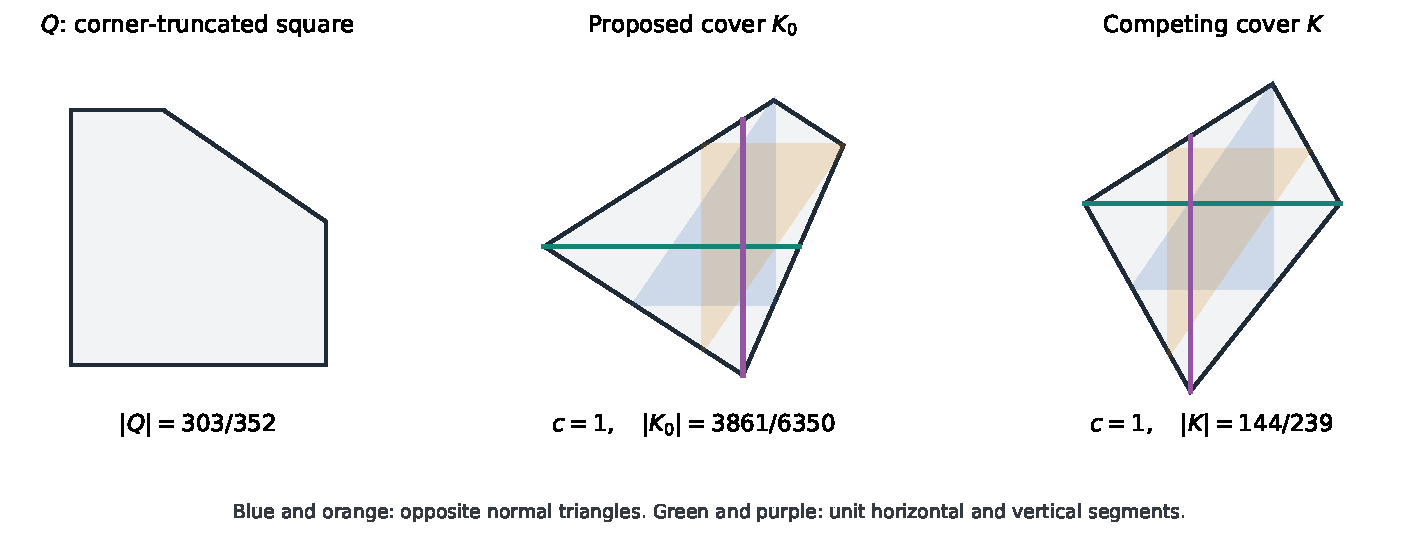
\includegraphics[width=\linewidth]{figures/truncated-covers.pdf}
 \caption{The corner-truncated square, the proposed partner, and the
 competing partner at the exact parameters $A=11/20$, $B=4/5$. The two
 cover panels use the same scale; each contains translations of the four
 unit normal templates.}
 \label{fig:truncated-covers}
\end{figure}
